\documentclass{article}
\usepackage[utf8]{inputenc}
\usepackage[T1]{fontenc}
\usepackage{microtype}
\usepackage{graphicx}
\usepackage{booktabs}
\usepackage{amsmath,amssymb,amsthm}
\usepackage{array}
\usepackage{placeins}
\usepackage{url}
\usepackage[hyperfootnotes=false]{hyperref}
\usepackage[preprint]{icml2026}
\hypersetup{pdftitle={Typed Incidence Graphs for Task-Conditioned Language Support},pdfauthor={Anonymous Authors},pdfsubject={Research prototype; repository audit and synthetic structural evaluation; not submitted or peer reviewed},colorlinks=true,urlcolor=blue,citecolor=blue,linkcolor=blue}
\icmltitlerunning{Typed Incidence Graphs for Language Support}
\icmlkeywords{typed incidence graphs, provenance, language learning, bounded queries, structural validation}
\newtheorem{proposition}{Proposition}
\newcommand{\Nabu}{\textsc{Nabu}}
\newcommand{\ind}{\mathbf{1}}
\newcommand{\artifact}[1]{\nolinkurl{#1}}
% Generated only from docs/graph-evaluation/results.json; do not edit numeric values.
\newcommand{\GraphAlignments}{1,026}
\newcommand{\GraphLanguages}{12}
\newcommand{\GraphTermSlots}{12,312}
\newcommand{\GraphTranslationPairs}{135,432}
\newcommand{\GraphRoleMismatches}{396}
\newcommand{\GraphNodes}{16,833}
\newcommand{\GraphFactors}{4,190}
\newcommand{\GraphSources}{4,199}
\newcommand{\GraphIncidences}{21,598}
\newcommand{\GraphForms}{12,706}
\newcommand{\GraphSnapshotBytes}{8,658,850}
\newcommand{\GraphExportBytes}{13,768,045}
\newcommand{\GraphRuntimeBytes}{934,444}
\newcommand{\GraphTopicPairs}{13,935}
\newcommand{\GraphBridges}{67}
\newcommand{\GraphAmbiguousKeys}{134}
\newcommand{\GraphMultipleRoles}{426}
\newcommand{\GraphOccurrenceCount}{24}
\newcommand{\GraphAcceptanceChecks}{24}
\newcommand{\GraphSubsets}{7,680}
\newcommand{\GraphConjunctionRows}{
1 & $0.0000 \pm 0.0000$ & $0.0000 \pm 0.0000$ \\
2 & $0.4863 \pm 0.0373$ & $0.6461 \pm 0.0449$ \\
4 & $0.8529 \pm 0.0218$ & $0.9149 \pm 0.0217$ \\
8 & $0.9798 \pm 0.0078$ & $0.9895 \pm 0.0052$ \\
16 & $0.9844 \pm 0.0000$ & $0.9921 \pm 0.0000$ \\
}
\newcommand{\GraphSizeRows}{
2 & 20,000 & 20,000 & 3.107 & 1.376 \\
4 & 40,000 & 120,000 & 3.885 & 8.253 \\
8 & 80,000 & 560,000 & 5.440 & 38.516 \\
16 & 160,000 & 2,400,000 & 8.551 & 165.067 \\
}

% Official ICML vendor files are unchanged. No affiliation or submission is invented.
\makeatletter
\renewcommand{\printAffiliationsAndNotice}[1]{%
  \global\icml@noticeprintedtrue%
  {\let\thefootnote\relax\footnotetext{\hspace*{-\footnotesep}%
  Anonymous research prototype. Not submitted or peer reviewed.
  Evaluation comprises repository measurements and synthetic structural cases.}}}
\makeatother

\begin{document}
\twocolumn[
\icmltitle{Typed Incidence Graphs for Task-Conditioned Language Support}
\begin{icmlauthorlist}
\textbf{Anonymous Authors}
\end{icmlauthorlist}
\vskip 0.3in
]
\printAffiliationsAndNotice{}

\begin{abstract}
A language graph should explain which recorded structure supports a proposed action without confusing connectivity, applicability, and learner knowledge. We develop an additive typed-incidence foundation for the existing \Nabu{} reader. Language-qualified forms, authored alignments, exact source occurrences, and task-material assertions remain distinct; complete applications retain all inputs, guards, provenance, and competing analyses. A pure kernel separates association discovery from conjunctive availability and returns versioned witnesses with explicit query bounds. We establish local preservation, projection-loss, provenance, and utility-identifiability results, then test the implemented contracts. The real catalogue contains \GraphAlignments{} authored alignments in \GraphLanguages{} languages: all \GraphTranslationPairs{} existing translation cases agree with the new query, while \GraphRoleMismatches{} target-role differences require explicit handling. On \GraphSubsets{} fixed-seed synthetic input subsets, the complete-application gate matches the declared conjunction oracle; flattened-edge reachability fails as arity grows and agrees in the unary control. Size and work-count experiments expose both incidence savings and metadata costs. These results support a verifiable retrieval foundation, not linguistic validation, learned relevance, or human learning benefit.
\end{abstract}

\section{Introduction}
\label{sec:introduction}

A learner may be preparing to meet a partner's mother, trying to understand a line of poetry, or reading with no destination beyond curiosity. The useful next action depends on that immediate activity. A language graph can organize relevant forms, interpretations, examples, and source passages. Its connections do not, by themselves, establish that an interpretation is correct, that a transformation applies, or that a learner needs practice.

This distinction becomes consequential when a small authored bank is extended toward richer linguistic structure. A word may participate in multiple readings; an expression may have separate literal and meaning renderings; a morphological operation may require several inputs and contextual conditions. Flattening these records into untyped edges loses distinctions that later algorithms cannot recover. Counting paths can also multiply copies of one source, while a highly connected topic may simply reflect how the catalogue was assembled.

We ask a deliberately operational question: \emph{What graph representation and query contract can support increasingly rich language structure while making the evidence for each returned material inspectable?} We answer it within an existing application. The implementation preserves legacy translation identities and exercise behavior, adds a typed incidence snapshot, and uses structural witnesses only for candidate discovery. Learner observations and action selection remain separate.

The contribution is an executable foundation with explicit limits: (i) a representation that retains role-bearing, source-qualified records and complete applications; (ii) local query and availability contracts with counterexamples to weaker interpretations; and (iii) a reproducible audit and synthetic evaluation covering compatibility, ambiguity, conjunction, provenance reuse, and work budgets. We do not propose a new general hypergraph algorithm, a validated ontology, or a model of human learning. The next step is small enough to verify now and structured enough to accept reviewed linguistic records later.

\section{Existing System and Relevant Foundations}
\label{sec:setting}

\paragraph{An extension of a working reader.}
\Nabu{} already contains a generated multilingual bank, curated reader media, exercises, a spaced-practice system, learner event storage, scoped intents, and a next-step selector. An intent distinguishes the immediate activity from an optional destination and preserves explicit, inferred, exploratory, and unknown information. A team objective remains separate from a member's private intent. The new graph does not store these private records. Its queries use explicit public structural seeds; the existing selector receives their answers alongside its separate intent and direct-evidence inputs.

The current bank contains \GraphAlignments{} authored alignment groups and \GraphTermSlots{} language slots. A legacy ``concept'' is such an alignment, not a verified multilingual lexeme. The graph adapter therefore keeps legacy IDs, language-qualified surface identities, and null lexeme/sense identities where no inventory exists. Reader annotations retain exact source-version and occurrence anchors. All current bank and curated content remain labelled authored and unreviewed.

\paragraph{Established mathematical representations.}
Directed hypergraphs provide a natural vocabulary for relations with multiple tails and heads \citep{gallo1993directed}. Factor graphs make arguments of local functions explicit through a bipartite representation \citep{kschischang2001factor}. We use the representational idea of first-class relation records and incidence ports; we do not run sum-product or treat the graph as a probabilistic learner model. A bipartite graph with retained factor records is sufficient for our purposes. The issue is information lost by a particular projection, not an inherent inability of ordinary graph storage to represent higher-order structure.

Provenance semirings distinguish ways of combining annotated data and show why dependency information should survive queries \citep{green2007provenance}. Our implementation is narrower: it preserves steps, source references, and declared lineage groups. It does not evaluate arbitrary provenance polynomials or infer source probabilities. Knowledge compilation also makes the tradeoff between representation size and supported queries explicit \citep{darwiche2002knowledge}. We accordingly specify the local queries we implement rather than asserting tractability for unrestricted global planning.

Learner models such as knowledge tracing \citep{corbett1994knowledge} and fitted recall-over-time models \citep{settles2016trainable} address different inferential questions. The production observation projector in this application retains bounded direct counts and a replayable ledger with \texttt{competence: null}. Structural availability supplies no observation likelihood and does not update those counts.

\section{Typed, Source-Qualified Incidence Structure}
\label{sec:representation}

\subsection{Records, Ports, and Identity}

Let a snapshot be $\mathcal{H}=(V,F,S,M,\tau,\rho,\nu)$, where $V$ contains entity records, $F$ relation records called factors, and $S$ source records. The type map $\tau$ distinguishes forms, authored alignments, usages, media, topics, and task profiles. Each factor $f$ retains a finite collection of complete ports
\begin{equation}
 M_f=\{(v,r,a):v\in V,\ r\text{ is a declared role}\},
\end{equation}
where $a$ contains any additional port attributes, such as language or position. Exact duplicate ports are rejected. A repeated endpoint in distinct roles is valid. Factor identity, type, status, semantics, and other payload fields are preserved. The map $\rho(f)\subseteq S$ names its source records; $\nu$ includes snapshot and source-version fingerprints.

The representation separates exact form identity from tolerant lookup. A surface ID uses a language tag and NFC-normalized text. Search may additionally fold case, strip punctuation, or apply the existing language-specific normalization. Such retrieval equivalence does not merge form records. A match can therefore return multiple authored alignments and roles without inventing a dictionary sense.

\begin{table}[t]
\caption{Distinct records answer distinct questions. These are current implementation types, not a complete linguistic ontology.}
\label{tab:types}
\centering\small
\begin{tabular}{@{}p{.25\columnwidth}p{.69\columnwidth}@{}}
\toprule
Record & Meaning and boundary \\
\midrule
Form & Exact language-qualified surface; not a lexeme. \\
Alignment & Existing authored grouping; not certified equivalence. \\
Usage / media & Authored example or exact source occurrence with version. \\
Association & Recorded membership or relation; no implication semantics. \\
Application & Whole inputs/outputs, features, guards, sources, alternatives. \\
Task material & Explicit authored material role; no measured utility. \\
\bottomrule
\end{tabular}
\end{table}

\begin{proposition}[Preservation relative to declared records]
For valid snapshots with unique identities, encoding every factor as a first-class record with its complete ports and payload admits reconstruction of the declared records, up to specified canonicalization. Forgetting factor identities or port roles need not admit reconstruction.
\end{proposition}
\begin{proof}
The incidence encoding stores each node and source record, each factor payload, and every port attached to that factor ID. Reading those records reconstructs the original collections; canonical sorting and deduplication of identical source references do not change their declared content. Conversely, one endpoint may have two roles in one factor, which an unlabelled edge cannot distinguish. Section~\ref{sec:applications} gives a second collision involving conjunction.
\end{proof}

This is a preservation statement, not a claim that the supplied records are true. The constructor rejects missing endpoints, unknown source references, conflicting identity reuse, and inconsistent application bindings. Identical records with the same ID are idempotent for the normalized snapshot and query answers; the duplicate audit counters can still change. Distinct source occurrences and claims retain distinct IDs.

\subsection{Whole Applications and Partial Context}
\label{sec:applications}

An application factor retains
\begin{equation}
 A_f=(I_f,O_f,\phi_f,G_f,P_f,\mathcal{A}_f),
\end{equation}
where $I_f$ and $O_f$ are complete input/output records, $\phi_f$ includes features and operation identity, $G_f$ is an explicit list of contextual guards, $P_f$ is provenance, and $\mathcal{A}_f$ contains complete competing analyses. Input/output IDs, forms, languages, and port roles must match the snapshot. An empty guard list explicitly declares no additional contextual requirement; an omitted list is invalid.

For supplied structural inputs $U\subseteq V$ and a partial context $c$, guard evaluation takes values in $\{\mathsf{true},\mathsf{false},\mathsf{unknown}\}$. A missing or null context value remains unknown. A different supplied value is a mismatch. Let $Q(f)$ denote eligibility under the explicit review and fixture policy. The implemented availability condition is
\begin{equation}
\begin{split}
 \operatorname{Avail}(f;U,c)={}&Q(f)\ \land\ (\mathcal{A}_f=\varnothing)\\
 &\land\ I_f^{\rm ids}\subseteq U
 \land\bigwedge_{g\in G_f}[g(c)=\mathsf{true}].
\end{split}
\label{eq:availability}
\end{equation}
Quarantined, unresolved, generated, or unknown records cannot silently become available. Authored applications and synthetic fixtures require explicit opt-in. Diagnostic statuses distinguish blocked, unresolved-analysis, context-mismatch, context-unknown, and missing-inputs. The tests use fictional forms and stipulated fixture statuses; no real morphology application is imported.

\begin{proposition}[Projection collision and activation error]
A projection retaining only edges from each input to each output cannot generally determine conjunctive availability. For one $k$-input application, if inputs are independently supplied with probability $p$, treating any path as availability has false-positive probability
\begin{equation}
 1-(1-p)^k-p^k.
\label{eq:projection-error}
\end{equation}
\end{proposition}
\begin{proof}
The complete rule $\{A,B\}\!\to\!C$ and two unary rules $A\!\to\!C$, $B\!\to\!C$ have the same projected edges. With $U=\{A\}$, only a unary rule is available. Thus no function of that projection and $U$ can be correct for both structures. In the single-rule probability example, the projected path test accepts whenever at least one input is supplied; the declared application accepts only when all are supplied. Their difference is the event ``neither zero nor all,'' giving Equation~\ref{eq:projection-error}.
\end{proof}

The local gate does not compose applications recursively or interpret $U$ as a learner's known skills. It also abstains whenever alternatives remain, even if they agree on the output. A later possible-world solver could recover some of those cases, but would need explicit compatibility rules and a different query contract. Flattening mutually exclusive analyses into one traversable graph is not that solver.

\subsection{Source Lineage Is Not Independent Evidence}

For a witness $w$, let $F(w)$ be its used factors and let $\ell(s)$ be a declared lineage ID, or unknown. We return both source references and
\begin{equation}
 D(w)=\bigcup_{f\in F(w)}\{\ell(s):s\in\rho(f),\ \ell(s)\ne\bot\},
\end{equation}
with unattributed references retained separately. A witness step must match actual ports of its named factor, including disambiguating attributes when endpoint and role are insufficient. Unused factors cannot be added merely to inflate provenance.

\begin{proposition}[Declared-copy invariance]
Adding references whose lineage IDs already occur in $D(w)$ does not increase $|D(w)|$. This does not establish independence among distinct lineage IDs.
\end{proposition}
\begin{proof}
Set union is idempotent. Statistical independence is a property of a joint probability distribution; neither the set operation nor a distinct label supplies such a distribution.
\end{proof}

This modest guarantee prevents a source copied into several records from becoming several counted lineages. It does not detect undeclared copying. General provenance semirings are not all idempotent; bag multiplicity and Boolean support have different meanings. Our returned witnesses are auditable record traces, not complete provenance algebra or evidence weights.

\section{Task-Conditioned Queries with Explicit Limits}
\label{sec:queries}

A generic query specifies seed IDs $Z$, allowed relation types $R$, depth $d$, fixture policy, and limits $B=(b_F,b_I,b_V,b_A)$ on counted factors, incidences, nodes, and answers. The kernel indexes incidences by endpoint and relation type. It discovers association records in deterministic order; application factors are never traversed as unary links. Each returned material carries a witness, review statuses, graph version, and an explicit statement that no learner evidence is transferred.

The result includes completeness relative to this exact relation/depth policy and a reason when a limit interrupts discovery. Completeness is not an assertion that the catalogue exhausts the language or that a reading is resolved. The specialized surface query reads the indexed count of known matches before applying answer limits. Its lazy descriptors and bounded alternative list preserve an ambiguous status and exact total, while reporting how many alternative IDs were omitted.

\begin{proposition}[Local query contract]
For a validated fixed snapshot, every returned witness step names actual factor ports and attached sources. The generic traversal's counted work satisfies
\begin{equation}
 W_F\le b_F,\quad W_I\le b_I,\quad W_V\le b_V,
 \quad |\operatorname{answers}|\le b_A.
\end{equation}
When a required discovery operation is prevented by a limit, the result reports incompleteness.
\end{proposition}
\begin{proof}
Witness construction checks each referenced factor and port, then derives source references from the used factor IDs. Each traversal counter is checked before its next increment, and the answer limit before insertion. The interrupted branch adds a reason and exits. Exhausting the allowed traversal exactly at a limit can remain complete because no additional operation was prevented.
\end{proof}

These are work-accounting guarantees, not universal latency guarantees. Index construction validates and clones supplied metadata and canonically sorts identities and ports. It must read the complete input; sorting costs are additional. Let $N=|V|$, $F_0=|F|$, $S_0=|S|$, and $I=\sum_f|M_f|$. Incidence storage has $I$ ports plus record payloads, while a directed clique expansion has $\sum_f k_f(k_f-1)$ edge records for $k_f$ distinct members. Record sorting includes $N\log N$, $F_0\log F_0$, $S_0\log S_0$, and $\sum_f k_f\log k_f$ comparison terms; comparison and cloning costs also depend on metadata size.

After indexing, the kernel merges pre-indexed lists for the requested relation types. Skipping already examined factors, copying bounded witness paths, and handling identifiers incur bookkeeping beyond the displayed counters. The specialized queries additionally validate bounded input text and current source anchors. No claim is made that setting \texttt{maxAnswers} alone bounds preprocessing or wall-clock time. Global alternative combinations can also grow rapidly: $g$ unconstrained binary analysis choices already permit $2^g$ assignments. We neither enumerate them nor claim that a local work budget solves their global consistency.

\paragraph{Relevance requires a task.}
A graph-only centrality score cannot identify arbitrary task utility. Fix a graph with materials $a,b$; one task can require $a$, another $b$. A deterministic ranking depending only on that unchanged graph must give the same order for both and cannot uniquely optimize both opposite utilities. Task constraints therefore enter discovery as explicit seeds and allowed relations. This does not validate a utility estimate: the current three introduction materials have authored task roles and preserve existing heuristic priorities. No learned score is produced by the graph.

\section{Implementation Boundary}
\label{sec:implementation}

The additive snapshot is assembled from existing generated bank records, curated content, source annotations, and a small authored task-material overlay. Topics become membership factors rather than new category cliques. Existing bridges retain their source distinctions, including category-generated anchors. The public kernel has no learner storage or model dependency. The adapter supports three concrete query families: surface-to-alignment witnesses, exact occurrence-to-source witnesses, and explicitly authored task-to-material witnesses.

The existing next-step layer consumes these answers for discovery. Its seven action contracts, direct-evidence interpretation, and heuristic scoring remain in place. Ambiguous or incomplete discovery does not become a confident single match. The change does not migrate cards, rewrite learner histories, generate linguistic facts from user text, or transmit intent text to an external model. Private learner state remains in the existing actor-scoped storage; this is not a new enterprise-isolation claim.

The full source, evaluation generator, saved results, tests, editable manuscript, and figure generator accompany the artifact. The prior observation/prediction/policy evaluation is unchanged and its checked paper is archived separately. We cite repository-derived measurements below by their reproducible artifact paths in Appendix~\ref{app:reproduction}.

\section{Evaluation}
\label{sec:evaluation}

We evaluate representation and structural query behavior. We do not fit a learner model, replace the scheduler, or compare instructional policies. In particular, exact translation compatibility is a software-contract oracle, not an independently reviewed linguistic benchmark.

\subsection{Protocol and Controls}

\paragraph{Catalogue audit.}
We reconstruct the typed snapshot, check canonical round-trip stability, query every existing directed language pair for every alignment, compare the returned translation contract with the existing translator, inspect target roles, and query every anchored reader annotation. Real cases include the two English ``light'' alignments, unknown text, and a one-answer ambiguity cap. The audit also records exact JSON bytes for the legacy explicit export, the typed snapshot, and the existing runtime module. They have different information content and are not interchangeable memory measurements.

\paragraph{Matched conjunction experiment.}
Both methods receive identical applications and supplied-input subsets. The complete gate is compared with reachability on the deliberately flattened input-to-output edges. An independent set-inclusion oracle defines correctness. We fix 12 seeds, arities $\{1,2,4,8,16\}$, and 128 subsets per seed/arity: one empty, one complete, and 126 keyed pseudorandom subsets with inclusion probability $1/2$. There are \GraphSubsets{} subsets and two assessed methods per subset. The unary case is a positive control, and the complete case prevents undefined recall. Under ideal independent fair draws, the expected all-case false-positive rate is $(126/128)(1-2^{1-k})$; the forced boundary cases are included in every denominator.

We report false positives divided by all subsets, false positives divided by claimed-available subsets, precision, and recall. Means and sample SD are across the 12 fixed-seed replicates. They are not human-population confidence intervals. The deterministic generator and full seed-level CSV are supplied.

\paragraph{Failure cases and scale.}
Ten declared application cases cover missing inputs, satisfied inputs, unknown/mismatched/satisfied context, alternatives, quarantine, generated status, and fixture/review opt-ins. Copy experiments use 1, 5, or 20 source records with one declared lineage. Relation-filter tests add 0, 10, 100, or 1,000 irrelevant topic factors. Width tests use one allowed factor with 100, 1,000, or 10,000 members and a fixed 16-incidence budget. Scale fixtures use 100, 1,000, or 10,000 association factors and arities 2, 4, 8, or 16. They report exact representation counts, JSON bytes, and kernel work counters, not wall-clock timings.

\begin{figure*}[t]
\centering
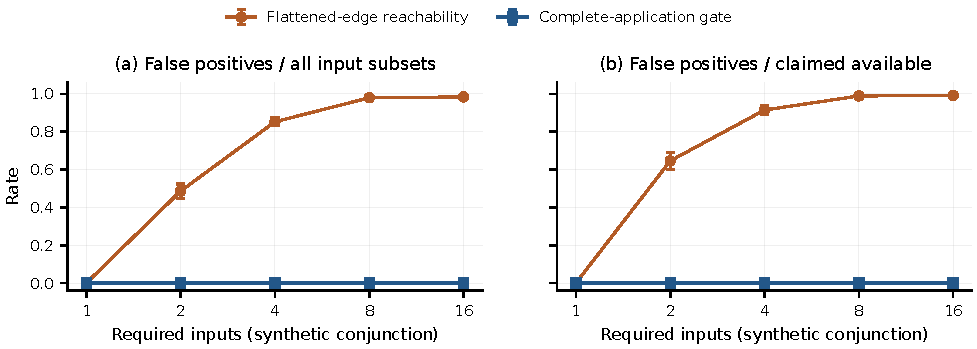
\includegraphics[width=.97\textwidth]{figures/graph_conjunction.pdf}
\caption{Matched synthetic conjunction checks. Both methods see identical supplied-input subsets. Flattened-edge reachability treats any supplied input as sufficient; the complete gate requires every declared input. Both agree in the unary control. Bars are sample SD across 12 fixed seeds, not confidence intervals about learners. The reference is the stipulated conjunction, not natural-language correctness.}
\label{fig:conjunction}
\end{figure*}

\subsection{Results}

\paragraph{Compatibility and real ambiguity.}
All \GraphTranslationPairs{} translation cases returned the existing output with zero missing alignment answers and zero contract mismatches. We found \GraphRoleMismatches{} cases where the previous structural adapter's listed target differed from the translator's actual output; the new witness selects the meaning-rendering role. For example, the bank distinguishes an original expression from its authored explanation. This fixes an interface-role inconsistency while preserving the translator; it does not certify either wording linguistically.

The snapshot contains \GraphNodes{} nodes, \GraphFactors{} association factors, \GraphSources{} source records, and \GraphIncidences{} ports. Of its nodes, \GraphForms{} are exact forms; none is promoted to a verified lexical sense. There are \GraphAmbiguousKeys{} ambiguous normalized lookup keys and \GraphMultipleRoles{} form/factor combinations carrying multiple roles. ``Light'' retains both known alignments when only one answer is returned. All \GraphOccurrenceCount{} reader annotations yield exact source witnesses with null bank-alignment, lexeme, and sense links. There are zero production application factors.

\paragraph{Conjunction succeeds only when preserved.}
The complete gate has zero false positives and zero false negatives on all generated subsets. The flattened baseline also agrees at arity one, but its all-case false availability rises from $.4863\pm.0373$ at arity two to $.9844\pm.0000$ at arity sixteen (Figure~\ref{fig:conjunction}). Both methods have recall one because all-input cases are reachable; recall alone conceals the projection's failure. These outcomes are expected from the declared semantics and Equation~\ref{eq:projection-error}. They test the implementation and expose the consequence of information loss; they do not establish superiority over lossless incidence graphs implemented with ordinary graph primitives.

All ten application gate cases return their predeclared status. The alternative-analysis case deliberately uses the same output under both analyses and still abstains. This is a coverage cost of the conservative contract: zero erroneous activation in these cases should not be read as complete inference.

\begin{figure*}[t]
\centering
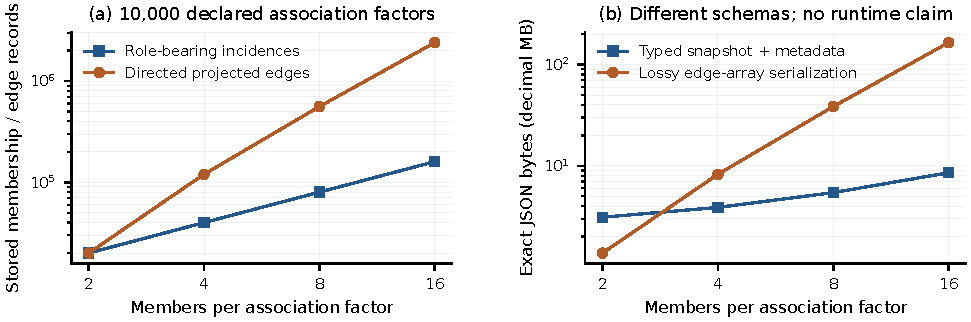
\includegraphics[width=.97\textwidth]{figures/graph_representation.pdf}
\caption{Measured representation counts and exact serialization sizes for 10,000 synthetic association factors. Incidences grow as $k$ per factor and directed projected edges as $k(k-1)$. The snapshot retains richer metadata, so it is larger at arity two. The projected array loses grouping and roles; the byte comparison is not an equal-information runtime benchmark. The current production runtime was already compact.}
\label{fig:representation}
\end{figure*}

\paragraph{Copies, distractors, and finite budgets.}
All source-copy settings preserve the separate references while returning one declared lineage and \texttt{independenceEstablished: false}. With the task-support filter, all four distractor settings return the same material and count exactly one factor, two incidences, and two nodes after indexing. Each wide-factor query visits sixteen incidences, returns sixteen answers, and reports incompleteness (Figure~\ref{fig:budgets}). These invariants depend on correct relation declarations; an irrelevant factor mislabelled as task support would pass that filter.

\paragraph{Incidence savings have boundaries.}
At 10,000 factors and arity sixteen, the fixture stores 160,000 incidences rather than 2,400,000 directed projected records. The complete snapshot is 8.551 decimal MB; the lossy projected array is 165.067 MB. At arity two, however, the snapshot is 3.107 MB while the projected array is 1.376 MB. Richer record metadata has a real cost, and small-arity cases do not yield a universal byte reduction.

The real legacy export contains \GraphTranslationPairs{} translation edges, \GraphTopicPairs{} topic pairs, and \GraphBridges{} bridge records, totalling \GraphExportBytes{} JSON bytes. The new snapshot is \GraphSnapshotBytes{} bytes. The existing runtime graph module is only \GraphRuntimeBytes{} bytes and did not require materializing that export. Therefore these measurements do not show an application-memory or latency improvement. They establish exact representation sizes and a route to avoiding future pair expansion.

The run passes \GraphAcceptanceChecks{} explicit evaluation acceptance statements. Regression testing also covers the kernel, adapter, recommendation integration, and existing application contracts; the current verification report, rather than a frozen count in this paper, records whole-repository totals.

\begin{figure*}[t]
\centering
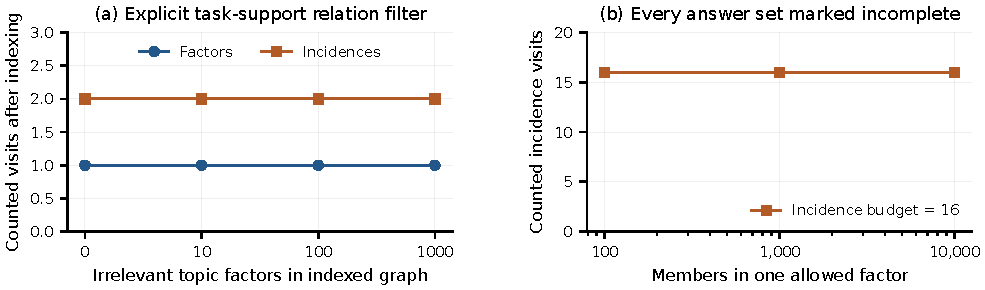
\includegraphics[width=.97\textwidth]{figures/graph_budgets.pdf}
\caption{Counted local query work after index construction. Left: irrelevant topic factors are excluded by the explicit relation filter. Right: a fixed incidence budget interrupts each wide allowed factor and marks the answer incomplete. These measurements exclude validation, sorting, source-text checking, and witness-copying costs; they are not latency measurements.}
\label{fig:budgets}
\end{figure*}

\section{Limitations and the Next Logical Step}
\label{sec:limits}

The strongest guarantees are deliberately about records and local execution. Source-grounded does not mean independently attested; the existing catalogue remains authored and unreviewed. A correct witness can trace a false claim. Exact source anchors can preserve an erroneous annotation. We preserve quarantine boundaries rather than allowing an attractive graph path to override them.

There is no production morphology inventory, verified multilingual lexeme system, global application solver, inferred source reliability, or automatic graph-to-learner transfer. Competing analyses remain unresolved, and no local path proves semantic equivalence, grammaticality, or learner readiness. The synthetic applications are fictional, and the baseline is an explicitly lossy projection. Their error rates are not empirical estimates for real morphology. Similarly, the topic experiment verifies a declared filter, not an ability to infer which relations a learner needs.

Scalability claims are conditional. The current snapshot is small enough for a browser but its metadata and indexing are not free. Wider deployments will require measured startup, memory, and query costs, incremental/versioned indexes, and a partitioning strategy that preserves source and ambiguity boundaries. More expressive reasoning should add explicit semantics and tractability analyses; it should not quietly reinterpret association paths as proofs. Our implementation makes neither global-optimality nor minimum-cost planning claims.

The immediate next step is to curate a small, independently reviewed set of complete applications and task-material relations, each with sources, applicability guards, counterexamples, and unresolved alternatives. Review should assess the \emph{whole application}, not count sibling suffixes as independent evidence. Hold out genuinely separate lexical families when testing any future transfer model. First evaluate whether queries retrieve and abstain correctly; then compare prediction on identical observations and questions; only then compare action policies at equal content and time budgets. Those are separate hypotheses.

For human evaluation, one unlaunched pilot proposal uses randomized parallel 12-minute sessions with the same reviewed Arabic content, estimator, and candidate pool, followed by an unassisted check targeting 48 hours within a predeclared 42--54-hour window. Scoring is blinded and task-specific, with a changed sentence and reviewed within-family/new-family probes where eligible. Declines and missing outcomes are retained. These durations are design choices, not validated optima; there is no sample-size, power, recruitment, or human-result claim.

\paragraph{Impact and governance.}
Keeping provenance and ambiguity visible can make errors easier to inspect, but does not remove them. Reviewers should be able to correct a source-specific claim without globally banning a legitimate form. Cultural and dialect differences require explicit contextual scope. Learner goals and team objectives remain private application state, not facts in a public language graph. No new external transmission or enterprise-security guarantee is introduced by this work.

\section{Conclusion}

The practical graph-first step is a typed, versioned incidence foundation with source witnesses and bounded local queries. It retains the information that richer linguistic reasoning would need, while preserving the existing reader and keeping learner inference separate. The audit verifies compatibility and exposes real role and ambiguity issues; controlled counterexamples show precisely where a forgetful projection fails and where the simpler unary case remains valid. The next advance should be better reviewed applications and explicit query semantics, followed by separately controlled prediction and policy studies. Connectivity alone does not supply those results.

\FloatBarrier
\bibliography{references}
\bibliographystyle{icml2026}
\appendix

\section{Artifact, Reproduction, and Version Boundaries}
\label{app:reproduction}

The artifact includes the complete application code and additive graph implementation, not a separate demonstration application. The graph-focused experiment and this manuscript can be reproduced without a paid API, credentials, production database, or network access after installing the normal local dependencies.

\begingroup\small
\begin{verbatim}
node tools/evaluate_graph.mjs \
  --output docs/graph-evaluation
node --test tests/graph-evaluation.test.mjs
python tools/build_graph_paper_figures.py
python tools/build_paper.py
\end{verbatim}
\endgroup

The recorded environment uses Node.js 24.22.1, Python with Matplotlib, and a local TeX installation. The repository build script can initialize an ignored local TeX cache if the installed distribution lacks one; it does not modify the system configuration. Official ICML 2026 style files are vendored unchanged. The paper is an anonymous research draft, not a submission or a course-grade claim. The main body is constrained to eight pages; references and appendices follow.

\begin{table*}[t]
\caption{Artifact map. The previous evidence experiment and archived paper remain separate from this structural evaluation.}
\centering\small
\begin{tabular}{p{.45\textwidth}p{.47\textwidth}}
\toprule
Path & Role \\
\midrule
\artifact{public/nabu-graph-kernel.js} & Pure typed incidence index, witnesses, bounded association traversal, full application gate. \\
\artifact{public/nabu-structure-query.js} & Current-source snapshot and surface, occurrence, task-material queries. \\
\artifact{data/task-material-relations.json} & Explicit authored overlay for three existing introduction materials. \\
\artifact{tools/evaluate_graph.mjs} & Fixed protocol, synthetic fixtures, complete compatibility audit, result generation. \\
\artifact{docs/graph-evaluation/results.json} & Full structured results, source hashes, fixtures, witnesses, acceptance statements. \\
\artifact{docs/graph-evaluation/results.csv} & Per-seed conjunction metrics and representation-size rows. \\
\artifact{docs/graph-evaluation/report.md} & Standalone explanation of measured results and limitations. \\
\artifact{tests/graph-evaluation.test.mjs} & Independent-oracle, fixture, byte-count, and reproducibility checks. \\
\artifact{tools/build_graph_paper_figures.py} & Vector figures and TeX numeric macros from saved results only. \\
\artifact{paper/figures/graph-manifest.json} & Figure source SHA-256, protocol, seeds, and error-bar semantics. \\
\artifact{paper/history/evidence-loop-20261114/} & Checked prior paper, source, bibliography, figures, and verification at commit \texttt{dd8e829}. \\
\artifact{docs/evidence-evaluation/} & Unchanged prior synthetic observation/prediction/policy experiment. \\
\bottomrule
\end{tabular}
\end{table*}

Results contain SHA-256 fingerprints for the evaluator, graph kernel, query adapter, graph modules, generated content/structure data, and source JSON files. The graph version binds authored sources and the listed semantic implementation dependencies. A policy-version string alone does not identify every implementation change; the reproducibility record preserves exact file hashes as well. The figure generator refuses a result with a failed acceptance statement and writes numeric macros directly from the saved JSON.

\section{Exact Experiment Definitions}
\label{app:protocol}

\subsection{Seeds and Identical Inputs}

The fixed seeds are 11, 29, 47, 83, 101, 137, 173, 211, 257, 307, 359, and 419. The generator uses a deterministic keyed integer hash to obtain values strictly between zero and one. Input inclusion is the threshold event $u<1/2$ keyed by seed, arity, trial, and input ID. It is pseudorandom fixture generation, not a claim of independent human sampling. Calls do not consume a shared random stream, so reordering other experiment cells does not change an input subset.

For every arity and seed, trial zero supplies no inputs and trial one supplies all inputs. Trials two through 127 use the keyed subset rule. The independent oracle checks whether the declared set of required IDs is contained in the supplied set. The typed method calls the actual production kernel with explicit fixture and authored opt-ins; the flattened baseline performs reachability using input-to-output edges without factor identities. Context and quality policies are identical and satisfied in this comparison. The separate gate cases vary them explicitly.

Let $y_t$ be the conjunction oracle and $\hat y_t$ the method's declared availability. We calculate
\begin{align}
 \mathrm{FP} &=\sum_t\ind[\hat y_t=1,y_t=0],\\
 \mathrm{FA} &=\mathrm{FP}/n,\\
 \mathrm{FCA} &=\mathrm{FP}/\sum_t\ind[\hat y_t=1].
\end{align}
Precision is $\mathrm{TP}/(\mathrm{TP}+\mathrm{FP})$ and recall is $\mathrm{TP}/(\mathrm{TP}+\mathrm{FN})$. The forced full-input case keeps both denominators positive for these methods. No probability forecast, Brier score, or calibration statistic is reported for this deterministic structural classification.

\begin{table}[ht]
\caption{Flattened-edge baseline: means $\pm$ sample SD across fixed seeds. The complete gate has zero false availability and unit precision/recall at every tested arity.}
\centering\small
\begin{tabular}{rcc}
\toprule
Arity & FP / all subsets & FP / claimed available \\
\midrule
\GraphConjunctionRows
\bottomrule
\end{tabular}
\end{table}

The SD is $\sqrt{\sum_{s=1}^{12}(m_s-\bar m)^2/11}$ for the metric $m_s$ computed within seed $s$. It describes variation across fixed generated replicates, not standard error or a confidence interval. At arity sixteen, the sampled random trials contain no all-present or all-absent extreme; the forced cases therefore explain the identical observed rates across seeds. This does not imply zero uncertainty in another distribution.

\subsection{Size Fixtures and Byte Accounting}

For each $(n,k)$ with $n\in\{100,1000,10000\}$ and $k\in\{2,4,8,16\}$, the generator creates $n$ nodes and $n$ association factors in a ring with a fixed seeded offset. Each factor has $k$ distinct members. The typed format includes schema/version fields, sources, fixture statuses, IDs, roles, and metadata. The illustrative projection emits an ordered pair record for every distinct member pair of every factor. It retains duplicate endpoint pairs arising from different factors, but omits factor identity, grouping, port roles, and most provenance. Deduplicating projected edges would lose additional information.

JSON byte counts are UTF-8 lengths with no pretty-printing. The projected array is counted by summing exactly serialized records and separators instead of allocating the whole quadratic array; a separate small test compares this computation with an independently materialized array. The current legacy export is small enough to materialize explicitly for its byte measurement. Neither representation is confused with JavaScript heap usage.

\begin{table*}[ht]
\caption{Exact counts and decimal MB for 10,000 synthetic factors. The two byte columns encode different information. All other size cells are in the CSV and JSON.}
\centering\small
\begin{tabular}{rrrrr}
\toprule
Arity & Incidence ports & Directed projected records & Typed snapshot MB & Lossy edge array MB \\
\midrule
\GraphSizeRows
\bottomrule
\end{tabular}
\end{table*}

The scale query uses one seed, depth one, and limits of 64 factors, 1,024 incidences, 256 nodes, and 64 answers. For the 10,000-factor rows, measured visits are respectively $(2,4,3)$, $(4,16,7)$, $(8,64,15)$, and $(16,256,31)$ for factors, incidences, and nodes. These regular ring cases remain within budget. The separate wide-factor tests force a 16-incidence interruption and preserve an explicit incomplete result.

\subsection{Source Copies, Topic Distractors, and Real Occurrences}

The copied-source fixture has two endpoint nodes and 1, 5, or 20 independently addressable association records. Each cites a different source ID with the same declared lineage. A witness explicitly names all used factor steps. Expected source-reference counts grow with copies; the lineage count remains one. There is no likelihood or confidence aggregation.

The distractor fixture has one task-support factor from a seed to a designated material. It adds 0, 10, 100, or 1,000 topic-membership factors, all incident on that seed. Their IDs sort before the relevant factor. A query allowing only task support returns the material with identical counted work. This construction tests typed adjacency rather than a favorable ID order. It supplies relevance by design and does not evaluate relevance inference.

The occurrence audit queries every current annotation by content ID, version, and annotation ID. Each answer must preserve its source anchor and null bank/lexeme/sense links. A same-spelling check uses distinct language-qualified IDs for English and German \emph{gift}; the fixture does not infer their meanings. Real polysemy is tested with the existing \texttt{home.light} and \texttt{colors.light} alignments. A cap of one preserves total matches two, ambiguous status, and the count of omitted alternative identities.

\section{Contract Details and Proof Boundaries}
\label{app:contracts}

\paragraph{Complete application validation.}
The retained application has its own ID, pattern ID, language, review status, fixture flag, all inputs and outputs with forms/languages/features, whole-operation features, provenance, and complete competing analyses. The factor additionally has typed ports and an explicit guard list. Input/output port ID sets must match their application parts; repeated ports cannot stand in for a missing required input. Validation of shape and binding does not validate linguistic correctness.

The gate first checks quarantine, status, and opt-in restrictions. It then reports unresolved alternatives, context mismatch, unknown context, missing inputs, or availability in that order. These diagnostic priorities do not change Equation~\ref{eq:availability}: only complete, eligible, unambiguous, context-satisfied records with every supplied input become available. No automatic output insertion, recursive closure, or learner update follows.

\paragraph{Witness scope.}
Each step contains a factor ID and two actual ports, including position or other distinguishing attributes when necessary. A witness may list seed nodes, but only its checked steps justify recorded relationships. Sources are derived from used factors, not from arbitrary graph proximity. A generic witness traces associations; the separate application witness includes every required input/output ID, features, guard results, and provenance. Neither establishes truth or independent evidence.

\paragraph{Canonicalization and duplicate boundaries.}
The constructor retains full JSON-compatible records, bounds nesting and record/port counts, rejects conflicting IDs, and clones/freezes its internal state. Canonical record ordering makes traversal reproducible under input ordering changes. Exact duplicate record IDs collapse for content; audit counters record their repetition. A changed factor payload under an existing ID is a conflict rather than a second vote. Distinct IDs do not prove distinct sources.

\paragraph{Alternatives and global reasoning.}
The implementation does not solve the set of all compatible analyses. For future reasoning, compatibility would need to say which alternatives are mutually exclusive, which guards apply, and what constitutes a valid composed derivation. Merely retaining alternatives is necessary for that extension but does not implement it. Our conservative abstention loses some answers, including the same-output case tested here. Enumerating paths or multiplying probabilities would not repair that missing semantics.

\paragraph{Task and learner identifiability.}
The centrality counterexample assumes task utility can differ while the language graph remains fixed. It rules out universal task optimization from topology alone under that assumption; it does not say topology is never useful as a feature. Similarly, supplied structural inputs in the application gate are query parameters, not estimates of learner mastery. Any future mapping from observations to latent state requires a separate model, assumptions, and held-out validation.

\section{Reviewed Expansion and One Unlaunched Pilot}
\label{app:pilot}

A defensible expansion would first add a bounded collection of independently reviewed applications and source-grounded task relations. Reviewers should record source versions, whole-operation applicability, dialect/register/context constraints, and competing analyses. Negative cases must include partial input sets, wrong domains, identical spellings with different readings, and conflicting sources. The graph evaluation should measure false availability, abstention, ambiguity preservation, and witness integrity before any evidence-transfer rule is proposed.

The existing human-pilot proposal is one study design, not multiple launched experiments. Parallel groups would receive randomized 12-minute sessions using the same independently reviewed Arabic content, estimator, and candidate pool, with fixed practice versus decision-sensitive support. A delayed unassisted check would target 48 hours in a predeclared 42--54-hour window, use a changed sentence, and include separate within-family and new-family probes only if reviewed eligible material exists. Blinded assessors would use a task-specific rubric rather than clicks or completion counts. Exact source versions, declined activities, missing follow-ups, and assistance would be recorded. Feasibility and variance estimates would inform a later sample-size decision; none is claimed here. Full details are in \artifact{docs/HUMAN_PILOT_PROPOSAL.md}.

This proposal would test an intervention, not retrospectively validate the graph's linguistic records or the current synthetic assumptions. The graph implementation is usable without conducting that study, and no recruitment, deployment, participant data collection, or efficacy claim accompanies the artifact.

\end{document}
